
\documentclass[twoside]{EPURapport}
\usepackage{listings}
\usepackage{algorithmic}
\usepackage{algorithm}
\usepackage{amssymb}
\usepackage{amsmath}

\renewcommand{\algorithmicrequire}{\textbf{Pr�condition:}}
\renewcommand{\algorithmicensure}{\textbf{Postcondition:}}
\renewcommand{\algorithmicend}{\textbf{fin}}
\renewcommand{\algorithmicif}{\textbf{si}}
\renewcommand{\algorithmicthen}{\textbf{alors}}
\renewcommand{\algorithmicelse}{\textbf{sinon}}
\renewcommand{\algorithmicelsif}{\algorithmicelse\ \algorithmicif} 
\renewcommand{\algorithmicendif}{\algorithmicend\ \algorithmicif} 
\renewcommand{\algorithmicfor}{\textbf{pour}}
\renewcommand{\algorithmicforall}{\textbf{pour tout}} 
\renewcommand{\algorithmicdo}{\textbf{faire}}
\renewcommand{\algorithmicendfor}{\algorithmicend\ \algorithmicfor} 
\renewcommand{\algorithmicwhile}{\textbf{tant-que}}
\renewcommand{\algorithmicendwhile}{\algorithmicend\ \algorithmicwhile} 
\renewcommand{\algorithmicloop}{\textbf{boucle}}
\renewcommand{\algorithmicendloop}{\algorithmicend\ \algorithmicloop} 
\renewcommand{\algorithmicrepeat}{\textbf{r�p�ter}}
\renewcommand{\algorithmicuntil}{\textbf{jusqu'�}}
\renewcommand{\algorithmiccomment}[1]{$/*$~#1~$*/$}
\floatname{algorithm}{Algorithme}
\renewcommand{\listalgorithmname}{Liste des algorithmes}
%\renewcommand{\lstlistlistingname}{Liste des codes}
%\renewcommand{\lstlistingname}{Code}

%\addextratables{%
%	\lstlistoflistings
%}

%\swapAuthorsAndSupervisors



\nolistoftables
\thedocument{Rapport de projet d'Algorithme et de Langage C}{Simulation du trafic urbain}{Simulation du trafic}

\grade{D�partement Informatique\\ 3\ieme{} ann�e\\ 2011 - 2012}

\authors{%
	\category{�tudiants}{%
		\name{Lei SHANG} \mail{lei.shang@etu.univ-tours.fr}
		\name{Yanxiao HU} \mail{yanxiao.hu@etu.univ-tours.fr}
	}
	\details{DI3 2011 - 2012}
}

\supervisors{%
	\category{Encadrants}{%
		\name{N�ron EMMANUEL} \mail{emmanuel.neron@univ-tours.fr}
	}
	\details{Universit� Fran�ois-Rabelais, Tours}
}

\abstracts{Le \textit{mod�le de conducteur int�lligent}(IDM) est un mod�le qui repr�sente l'action des conducteurs, c'est-�-dire le mouvement raisonable des voitures dans un trafic urbain. Nous avons �tabli l'algorithme � partir de ce mod�le pour simuler visuellement sur l'�cran, une file de voiture sur la route avec 2 feux de circulation. L'application que nous avons r�alis� peut �tre fortement configurable � l'aide du ficher de configuration.}
{IDM, Simulation du trafic, Algorithme, OpenGL}
{The \textit{Intelligent driver model}(IDM) is a time-continuous car-following model for the simulation of freeway and urban traffic. According to this model, we have proposed an algorithm and then an application to simulate traffic on the screen. This application is developped with C programming language and can be highly custumized with the help of the configuration file.}
{IDM, Traffic simulation, Algorithm, OpenGL}


\begin{document}

\chapter{Introduction}
Ce projet est d�velopp� dans le cadre de la formation de l'algorithme et le langage C en troisi�me ann�e du d�partement informatique. Le but du projet est de pratiquer les connaissances que nous avons acquises durant les s�ances de cours. 


Pour cela, nous sommes demand�s � d�velopper une application avec langage C pour simuler le trafic urbain, une file de voiture avec 2 feux de circulation. Donc il nous faut �tudier � la fois :
\bigskip
\begin{itemize}
	\item Le mod�le math�matique du mouvement des voitures sur la route
 	\item L'algorithme pour visualiser le mod�le ci-dessus 
 	\item La r�alisation langage C de l'algorithme ci-dessus (Nous avons choisi le technique OpenGL pour le r�aliser)
\end{itemize}
\bigskip


Notre travail, ainsi que ce rapport, est organis� selon ces trois parties.


\chapter{IDM (Intelligent Driver Model)}
IDM est un mod�le de la simulation du trafic urbain. Il est d�velopp� par Treiber, Hennecke and Helbing en 2000 pour am�liorer les mod�les existants qui ont moins de propri�t�s r�elles.

\section{D�finition}

$
\frac{dv}{dt}=a\left[1-\left(\frac{v}{v_{0}}\right)^{\delta}-
												\left(\frac{s^{*}}{s}\right)^{2}\right] \\
s^{*}=s_{0}+vT+\frac{v\Delta v}{2\sqrt{ab}}
$

L'architecture d'Android se compose de 4 couches. Elles sont la couche d'application, le cadre de l'application, les biblioth�ques et le noyau Linux. La figure \ref{fig:ch1_architechture} montre les principaux composants du syst�me d'exploitation Android.
\begin{figure}[h]
	\centering
	\includegraphics[width=14cm]{pics/ch1_architechture.png}
	\caption{\label{fig:ch1_architechture}Architechture du syst�me Android\protect\footnotemark}
\end{figure}
\footnotetext{\url{http://developer.android.com/guide/basics/what-is-android.html}}

\subsection{Caract�ristique}
Android fournit un ensemble d'applications de bases, y compris un client email, une application SMS, un calendrier, une carte, un navigateur, etc.

\subsection{Cadre de l'application}
En fournissant une plateforme de d�veloppement ouvert, Android offre aux d�veloppeurs la possibilit� de cr�er des applications extr�mement riches et innovantes. Les d�veloppeurs sont libres de profiter du mat�riel p�riph�rique, d'obtenir les informations de la position g�ographique, d'ex�cuter les services d'arri�re-plan, d'ajouter des notifications � la barre d'�tat, etc.


Les d�veloppeurs ont un acc�s complet aux APIs utilis�s par les applications de noyau. L'architecture d'application est con�ue pour la r�utilisation des composants. 

Toutes les applications sont une collection des services, y compris : 
\bigskip
\begin{itemize}
	\item Une collection riche de \textit{View} qui peuvent �tre utilis�e pour construire une application, y compris des listes, des grilles, des zones de texte, des boutons et m�me un navigateur web � embarquer.
 	\item Des \textit{Content Providers} qui permettent aux applications d'acc�der aux donn�es provenant d'autres applications (tels que les \textit{Contacts}), ou de partager leurs donn�es.
 	\item Un \textit{Resource Manager} qui offre l'acc�s aux ressources comme les cha�nes de caract�res localis�es, les graphiques, et les fichiers de mise en page.
 	\item Un \textit{Notification Manager} qui permet toutes les applications � afficher des alertes personnalis�es dans la barre d'�tat.
 	\item Un \textit{Activity Manager} qui g�re le cycle de vie d'application et fournit une pile de navigation.
\end{itemize}

\subsection{Biblioth�ques}
Android comprend une collection de biblioth�que de C ou C++ utilis� par les composants diff�rents. Ces capacit�s sont fournies par le cadre d'application Android. Certaines de ces biblioth�ques de noyau sont montr�es ci-dessous:
\bigskip
\begin{itemize}
	\item System C library - une impl�mentation de la biblioth�que C standard du syst�me (libc).
 	\item Media Libraries - bas� sur OpenCORE de PacketVideo. Des biblioth�ques permettent l'enregistrement audio et vid�o, ainsi que des fichiers d'images, y compris MPEG4, H.264, MP3, AAC, AMR, JPG et PNG. 
 	\item Surface Manager - g�re l'acc�s au sous-syst�me d'affichage
 	\item LibWebCore - c'est un moteur de navigateur moderne qui alimente le navigateur Android et une Web View embarqu�. 
 	\item SGL - le moteur graphique 2D. 
 	\item 3D Libraries - une impl�mentation bas�e sur OpenGL ES 1.0 APIs; les biblioth�ques utilisent l'acc�l�ration mat�rielle 3D (si disponible) ou le logiciel 3D optimis� hautement.
 	\item SQLite - un moteur de base de donn�es relationnelles puissant et l�ger � la disposition pour toutes les applications.
\end{itemize}

\subsection{Phase d'ex�cution Android}
Android comprend une collection des biblioth�ques de noyau qui offrent la plupart des fonctionnalit�s disponibles du langage Java.


Chaque application Android s'ex�cute dans son propre processus, avec sa propre machine virtuelle Dalvik. Dalvik est con�ue pour qu'un mat�riel puisse ex�cuter efficacement plusieurs machines virtuelles en m�me temps. Le VM Dalvik ex�cute les fichiers de format ex�cutable Dalvik (.Dex), qui est optimis� pour la minimale d'occupation m�moire. Le VM Dalvik d�pend le noyau Linux pour les fonctionnalit�s de bas-niveau comme le management de la m�moire.

\subsection{Noyau Linux}
Android est bas� sur le noyau Linux 2.6 pour les services du syst�me noyau, tels que la s�curit�, la gestion de la m�moire, la gestion des processus, etc. Le noyau est regard� comme une couche d'abstraction entre le mat�riel et le reste de la pile logicielle.

\section{Fonctionnement des applications Android}
Toutes les applications Android sont �crites en langage Java. Les outils du SDK Android compile le code --- avec toutes les donn�es et les fichiers de ressources --- dans un package Android, un fichier d'archive avec un suffixe \textit{.apk}. Tout le code dans un seul fichier \textsl{.apk} est consid�r� comme une seule application.


Quand install� sur un mat�riel, l'application Android vit dans sa propre boite de s�curit�:
\bigskip
\begin{itemize}
	\item Le syst�me d'exploitation Android est un syst�me multi-utilisateurs, sous lequel chaque application est un utilisateur diff�rent.
 	\item Par d�faut, le syst�me attribue � chaque application un ID utilisateur Linux qui est utilis� uniquement par le syst�me et qui est inconnu pour l'application. Le syst�me d�finit les autorisations de tous les fichiers de l'application, pour que seulement les utilisateurs qui ont le droit peuvent y acc�der.
 	\item Chaque processus a sa propre machine virtuelle (VM), donc l'application fonctionne s�par�ment.
 	\item Par d�faut, chaque application s'ex�cute dans son propre processus Linux. Android d�marre le processus lorsqu'un composant de l'application doit �tre ex�cut�, et arr�te le processus quand il n'est plus n�cessaire ou quand le syst�me doit r�cup�rer la m�moire pour d'autres applications.
\end{itemize}
\bigskip

Une application Android se compose d'une collection des composants. Il y a 4 composants principaux : \textit{Activity}, \textit{Service}, \textit{ContentProvider}, \textit{BroadCast receiver}. 

\section{Environnement de d�veloppement}
%Dans cette partie, nous pr�sentons l'environnement du travail, \textcolor{red}{qui inclut les outils mat�riels et les outils de d�veloppement (logiciels et technologies exploit�s)}.


\begin{description}
	\item[Installation de JDK] \hfill \\ On d�veloppe l'application Android avec le langage Java, donc le JDK est essentiel. Dans ce projet, nous utilisons le JDK version 6, qui peut �tre t�l�charg� du site officiel\footnote{\url{http://www.oracle.com/technetwork/java/javase/downloads/index.html}}.
	
	\item[Installation de SDK Android] \hfill \\ Nous avons t�l�charg� le SDK Android depuis le site d�veloppeur Android\footnote{\url{http://developer.android.com/sdk/index.html}}. Puis, nous les avons extraits sous le r�pertoire \verb?C:\Program Files\android-sdk-windows?.
	
	\item[Installation de Eclipse] \hfill \\ Eclipse est un IDE gratuit tr�s c�l�bre dans le domaine informatique. On peut le t�l�charger � partir du site Eclipse, la version \textit{Eclipse IDE for Java Developers}est recommand�e\footnote{\url{http://www.eclipse.org/downloads/packages/eclipse-ide-java-developers/indigosr2}}.
	
	\item[Installation de ADT] \hfill \\ Dans Eclipse, cliquer par s�quence : help $\rightarrow$ Install New software $\rightarrow$ Add, puis remplir les champs en fonction de la figure\ref{fig:ch1_addrepository}:\\
		
		\begin{figure}[h]
		\centering
		\includegraphics[width=10cm]{pics/ch1_addrepository.jpg}
		\caption{\label{fig:ch1_addrepository}Installation de ADT - Add repository}
		\end{figure}
		
		
		Apr�s cliquer sur ''OK'', Eclipse affiche les plugins disponiblies. Nous s�lectionnons le ''Android DDMS''(Android Dalvid Debug Moniter Server) et le ''ADT''(Android Development Tools). Nous validons les �tapes suivantes et nous red�marrons Eclipse pour finir l'installation des plugins. Maintenant on peut trouver les param�tre Android ici : Windows $\rightarrow$ Preferences $\rightarrow$ Android.
		
		\begin{figure}[h]
		\centering
		\includegraphics[width=10cm]{pics/ch1_preferences.jpg}
		\caption{\label{fig:ch1_preferences}Preferences Android}
		\end{figure}
	
	
	\item[Configuration de SDK] \hfill \\ Sous le menu Windows $\rightarrow$ Android SDK Manager, on peut s�lectionner et installer les paquets n�cessaires. Dans notre cas, API version 2.3 est suffisante. Ce qu'il faut faire attention, c'est que la version API doit �tre support� par l'appareil cibl�.
	
		\begin{figure}[h]
			\centering
			\includegraphics[width=10cm]{pics/ch1_androidsdkmanager.jpg}
			\caption{\label{fig:ch1_androidsdkmanager}Android SDK Manager}
		\end{figure}


	\item[Configuration de AVD] \hfill \\ Pour tester notre application pentant le d�veloppement, on peut utiliser directement notre portable Android, ou bien la lancer dans un appareil virtuel(AVD). Pour ce dernier, on peut lancer le gestionnaire AVD sous le menu \textit{Windows}, et cr�er un nouveau AVD en pr�cisant les param�tre. 

%\\[\intextsep]
%\begin{minipage}{\textwidth}
%\centering
%\includegraphics[width=8cm]{pics/ch1_createavd.jpg}
%\label{fig:ch1_createavd}
%\end{minipage}
%\\[\intextsep]
		\begin{figure}[!h]
			\centering
			\includegraphics[width=8cm]{pics/ch1_createavd.jpg}
			\caption{\label{fig:ch1_createavd}Cr�ation d'un AVD}
		\end{figure}


\end{description}

\chapter{Algorithme de l'application}
IDM est un mod�le qui est bas� sur l'�tat, c'est-�-dire quand on pr�cise un moment, on peut d�terminer les �tats (position, vitesse...) des voiture, et donc on peut afficher les voiture sur l'�cran. Ce que l'on a besoin, c'est seulement une boucle o� on mettre � jour les positions des voitures sur l'�cran. A partir de cette id�e, nous avons �tabli deux structures n�c�ssaires et l'algorithme principale.


Les structures de voiture et de la configuration sont d�finies ci-apr�s:
\begin{lstlisting}
nouvelle structure Config
{
    /** Param�tres pour l'affichage */
     windowWidth:entier;
    windowHeight:entier;
       roadWidth:r�el; 
        carWidth:r�el; 
       carLength:r�el; 
     
    /** (Longueur(m) virtuelle de la route/windowWidth(pixel). */
    roadVirtualLengthFactor:r�el; 
    
    /** Param�tres fonctionals */
    v0:r�el; /**La vitesse d�sir�e(km/h)*/    
     T:r�el; /**Temps de r�action*/
    s0:r�el; /**Gap minimal*/
     a:r�el; /**Acc�l�ration*/ 
     b:r�el; /**D�c�l�ration*/
};

nouvelle structure Car
{
    x:r�el; /**La postion courante*/
    v:r�el; /**La vitesse courante*/
    a:r�el; /**L'acc�l�ration*/
};
\end{lstlisting}

Et les algorithmes que nous avons cr��s sont d�crits au-dessous. Le premier est l'algorithme fondamental, qui d�crit le proc�dure d'ex�cution de l'application enti�re.
%Algo main
\begin{algorithm}[H]
\caption{Algorithme fondamental de l'affichage des voitures}
\label{algo:main}
\algsetup{indent=3em}
\begin{algorithmic}[1]
\REQUIRE { entr�es : config : Config initialis� du fichier de Configuration, \\
\makebox[40mm]{  }cars : un tableau de Car initialis�}
\ENSURE { sortie : Une file de voiture simul�e sur l'�cran }
%\STATE ini
\WHILE[La boucle qui dure jusqu'� la fin]{vrai} 
\STATE Dessiner l'arri�re plan
\FORALL{car dans le tableau Cars}
\STATE Dessiner la voiture sur l'�cran
\ENDFOR
\STATE Mettre � jour les param�tres des voitures pr�sent�s par cars
\ENDWHILE
\end{algorithmic}
\end{algorithm}


Algorithme ci-dessous est un sous-algorithme qui pr�sente le moyen de renouvellement des param�tres des voitures.
%Algo updateCars
\begin{algorithm}
\caption{Sous-algorithme pour renover les param�tres des voitures}
\label{algo:updatecars}
\algsetup{indent=3em}

\begin{algorithmic}
\REQUIRE { entr�es : cars : un tableau de Car}
\ENSURE { sortie : Le m�me tableau des voitures avec les param�tres renouvel�s.}
\FORALL{car dans le tableau Cars}
	\STATE Mettre � jour la position $x$ des voitures
	\STATE Mettre � jour la vitesse $v$ des voitures
	\STATE /* C'est la partie la plus importante, qui signifie l'action du conducteur intelligent et qui applique le mod�le IDM */
	\STATE Mettre � jour l'acc�l�ration $a$ des voitures
\ENDFOR

\end{algorithmic}
\end{algorithm}


L'algorithme suivant est la partie du coeur, qui applique le mod�le IDM. C'est un sous-algorithme plus d�taill� sur la m�thode pour mettre � jour le param�tre de l'acc�l�ration.
%Algo updateAcceleration
\begin{algorithm}[H]
\caption{Sous-algorithme pour mettre � jour le param�tre de l'acc�l�ration}
\label{algo:updateAcce}
\algsetup{indent=3em}
\begin{algorithmic}[1.1.1]
\REQUIRE { entr�es : cars : un tableau de $n$ Car,\\
\makebox[33mm]{  }config : Config initialis� du fichier de Configuration}
\ENSURE { sortie : Le m�me tableau des voitures avec les param�tres d'acc�l�ration renouvel�s.}
\FOR{i de $1$ � $n-1$}
	\STATE $car[i].a\leftarrow config.a
	\left[1-\left(\frac{car[i].v}{config.v_{0}}\right)^4-
		\left(
			\frac{config.s_{0}+car[i].v*config.T+\frac{car[i].v*(car[i].v-car[i+1].v)}{2\sqrt{config.a*config.b}}}{car[i+1].x-car[i].x}
		\right)^{2}
	\right]$
\ENDFOR

\end{algorithmic}
\end{algorithm}

\chapter{OpenGL}
Apr�s effectuer la premi�re partie de travail sur l'algorithme, nous passons � la suite pour la r�alisation de l'application. D'apr�s le but de ce projet, nous choisissons langage C pour la r�alisation. Cependant, ce que l'on veut faire, c'est de la programmation graphique, qui ne peut pas �tre r�alis�e en utilisant simplement ce que l'on a �tudi� pendant le cours. Alors nous avons fait de la recherche pour trouver une solution. Enfin nous avons choisi le technique OpenGL pour le faire.

\section{Introduction}
OpenGL(Open Graphics Library) est une librairie multiplate-forme qui d�finit un ensemble d'API pour faciliter la conception de l'application qui concerne les graphiques 3D/2D. Par rapport � DirectX(l'autre technique similaire sorti par Microsoft), OpenGL supporte plusieurs plate-formes. Par cons�quent elle est d�j� le standard de l'industrie. Elle contient environ 250 fonctions qui peuvent �tre utilis�es pour afficher des sc�nes trimentionnelles complex � partir des simples primitives g�om�triques.


Puisque OpenGL est simplement un ensemble des fonctions, elle seule ne nous permet pas de cr�er une fen�tre pour montrer notre application. Donc il existe plusieus extensions d'OpenGL qui fournit d'autres fonctionnalit�s. GLUT(OpenGL Utility Toolkit) est un bon choix.


\section{Environnement de d�veloppement}
Pour r�aliser cette application, nous avons choisi CodeBlocks comme notre outil de d�veloppement. Pour �tablir l'environnement de OpenGL, nous avons suivi les d�marches suivantes:

\begin{enumerate}
	\item T�l�charger et installer CodeBlocks.
	\item T�l�charger les fichers de GLUT.
	\item Placer glut32.dll � \verb�c:\windows\system�; glut32.lib � \verb�c:\program files\mingw\lib�, et
glut.h � \verb�c:\program files\mingw\include\GL�. Ce sont tous les positions par d�fault, en principe, les fichers *.dll doit toujours �tre plac� sous le r�pertoire syst�me Windows; les *.lib et *.h sont mis respectivement sous les r�pertoire de librairie et de ficher d'en-t�te du compilateur.
	\item Dans CodeBlocks, cr�er un nouveau projet GLUT et poursuivre les d�marches.Figure\ref{fig:ch3_newglut}
	\item Enfin on obtient un projet d'exemple, mais on doit quand m�me ajouter quelques choses pour le faire marcher. Ajouter \verb%#include<windows.h>% au d�but du ficher Main.
	\item Maintenant on peut d�j� lancer cet application d'exemple. Figure\ref{fig:ch3_glexemple}
\end{enumerate}	

\begin{figure}[!ht]
	\centering
		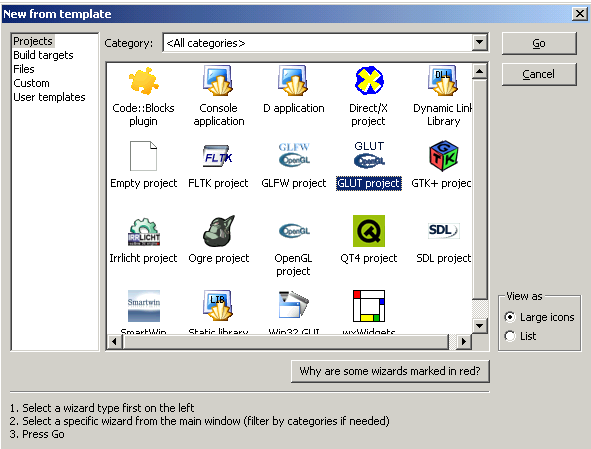
\includegraphics[width=14cm]{pics/ch3_newglut.png}
	\caption{Nouveau projet GLUT}
	\label{fig:ch3_newglut}
	\end{figure}
	
	\begin{figure}[!ht]
		\centering
			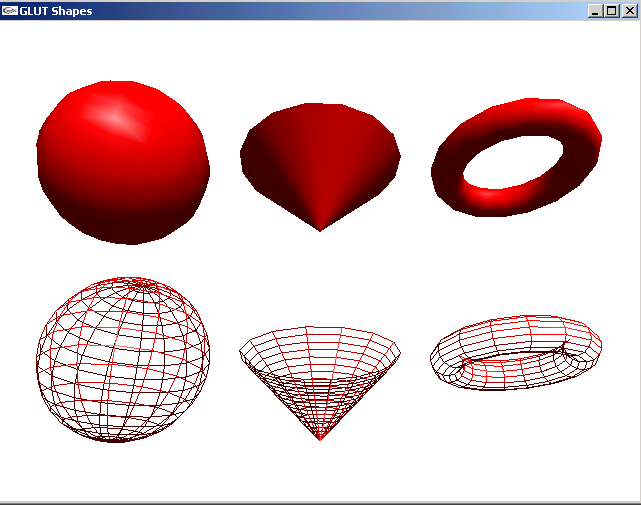
\includegraphics[width=14cm]{pics/ch3_glexemple.png}
		\caption{Exemple projet GLUT}
		\label{fig:ch3_glexemple}
	\end{figure}
	
\section{Structure d'une application OpenGL}
\label{ch3_structureopengl}
Pour ma�triser OpenGL, beaucoup de conna�ssances sont n�cessaires, mais ici, on peut quand m�me montrer une structure d'une application simplifi�e OpenGL.


La fonction main est g�n�ralement comme �a:
\begin{lstlisting}
int main(int argc, char** argv)
{
    glutInit(&argc,argv);
    glutInitDisplayMode(GLUT_DOUBLE| GLUT_RGB);
    glutInitWindowSize(config.windowWidth,config.windowHeight);
    glutInitWindowPosition(0,0);
    glutCreateWindow(''Traffic Simulation'');
    glClearColor(25.0/255,134.0/255,19.0/255,0.3);//Couleur de l'arri�re plan
    glShadeModel(GL_SMOOTH);
    /*Function callback. Fonction myReshape sera invoqu� 
     *quand la fen�tre change sa forme.*/
    glutReshapeFunc(myReshape);
    /*Fonction myDisplay actualiser l'�cran*/
    glutDisplayFunc(myDisplay);
    /*mouse est invoqu� quand un bouton de la souris est appuy�*/
    glutMouseFunc(mouse);

    /*Cr�er un menu*/
    glutCreateMenu(menuFonc);
    glutAddMenuEntry(''Start'',MENU_START);
    glutAddMenuEntry(''Renew configuration'',MENU_RENEW);
    glutAddMenuEntry(''Synchronize the traffic lights'',MENU_SYNC);
    glutAttachMenu(GLUT_RIGHT_BUTTON);//Lier ce menu avec un bouton
    
    /*Cette derni�re ligne commence la boucle principale de cet application*/
    glutMainLoop();
}
\end{lstlisting}

\chapter{Mise en oeuvre}
\section{Structure des fichers du projet}
Dans le premier temps, nous avons cr�er une version simplifi�e de notre application, simplement pour avoir une impression d'OpenGL. Ensuit, nous avons con�u � nouveau la structure du projet pour ajouter les autres fonctionnalit�s et aussi pour la clart�.


A la fin, notre projet a une structure comme Figure\ref{fig:ch4_filestructure}.
	\begin{figure}[!ht]
		\centering
			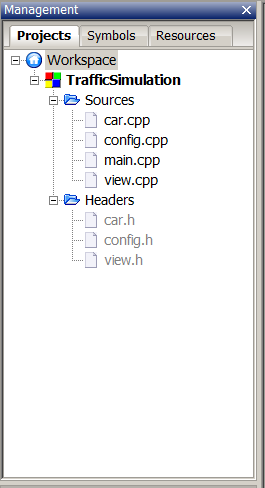
\includegraphics[width=7cm]{pics/ch4_filestructure.png}
		\caption{Structure des fichers}
		\label{fig:ch4_filestructure}
	\end{figure}
	
Les fonctions des fichers sont organis�s selon l'id�e de module. Les explications des fichers sont pr�sent�es ci-apr�s.
\bigskip
\begin{description}
	\item[config.c(.h)] \hfill \\ Il concerne les d�finitions et les op�rations par rapport � la configuration. La fonction principale dans cette partie est la fonction \textit{void initConfigurationFromFile(Config* c)}, qui, comme l'indiquer dans le nom de la fonction, sert � initialiser la configuration de l'application � partir d'un ficher.
	\item[car.c(.h)] \hfill \\ Il contient les d�finitions et les op�rations qui concernent la structure \textit{Voiture}. Nous avons aussi d�fini une structure de la liste des voiture, et les autres fonctions telle que \textit{carIn, carOut} correspondent � l'�v�nement d'entr�e et de sortie d'une voiture de la fen�tre.
	\item[view.c(.h)] \hfill \\ Ce ficher contient toutes les fonctions n�c�ssaires pour l'affichage, y compris les fonctions principales OpenGL. Par exemple, les fonctions indiqu�es dans la section \ref{ch3_structureopengl}, \textit{myResharp, myDisplay, mouse, menuFonc}, etc.
	\item[main.c] \hfill \\ Le ficher qui contient la fonction \textit{main} qui a une structure typique OpenGL pr�sent�e dans le chapitre pr�c�dent.
\end{description}	
	
\section{Interface de l'application}
Puisque le but du projet concerne plut�t l'algorithme et le langage C, alors nous n'avons pas attach� beaucoup d'importance sur la beaut� de l'interface. Une fois que l'interface peut donner une impression d'une file de voitures qui circule, c'est suffisant.


Alors, voir ci-dessous, l'interface de notre application.
	\begin{figure}[!ht]
		\centering
			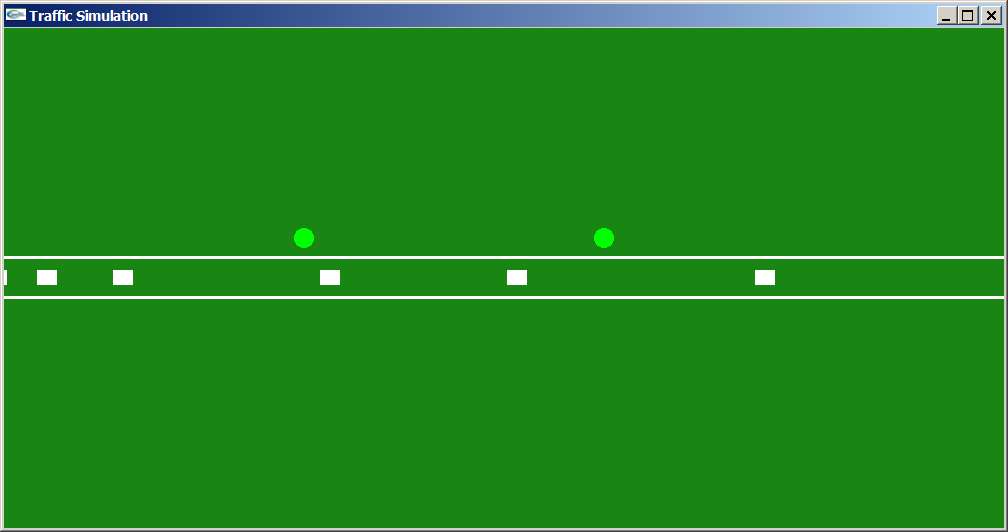
\includegraphics[width=14cm]{pics/ch4_interface.png}
		\caption{Interface de l'application}
		\label{fig:ch4_interface}
	\end{figure}
	

\section{Utilisation de l'application}
\subsection{Ficher de configuration}
Le ficher de configuration nomm� \verb{TS_setting.ini{ se trouve sous le r�pertoire \verb�C:\�. On peut changer les param�tres selons besoins, m�me pendant l'ex�cution de l'application. Les param�tres poss�dent un nom clair, les significations sont expliqu�es dans le ficher. L'unit� concernant la distance est pixel, et ce qui concerne le temps est milliseconde. Le suivant est le contenu de ce ficher initislis�.

\begin{lstlisting}
#The first two parameters about the window are used for 
#the initialisation of the window, so they should not be
# changed during the runtime
#time unit:ms
windowWidth=1000
windowHeight=500

roadWidth=40
carWidth=15
carLength=20

#The position of traffic lights is specified by their
#proportion to the window width
trafficLightPosition1=0.3
trafficLightPosition2=0.6
lightDurationWhenSynchronized=5000;
lightChangeDelayWhenSynchronized=-1;

#Parameters of the traffic
v0=500
v_begin=50
#unit:s
T=1.5
s0=2
a=30
b=6
#This value should not be too large, because if
#there is no car moving on the screen, openGL will stop refresh it.
moyen=1000
\end{lstlisting}


\subsection{Fonctionnalit�}

\begin{description}
	\item[Cliquer-droit$\rightarrow$ Start]  \hfill \\Faire entrer la file de voitures.
	\item[Cliquer-droit$\rightarrow$ Renew configuration] \hfill \\Renouveler les configurations de l'application apr�s que l'on a chang� le ficher de configuration.
	\item[Cliquer-droit$\rightarrow$ Synchronize the traffic lights] \hfill \\Synchroniser les deux feux.
	\item[Appuyer bouton 1] \hfill \\Arr�ter la synchronisation des feux et basculer le premier feu. 
	\item[Appuyer bouton 2] \hfill \\Arr�ter la synchronisation des feux et basculer le deuxi�me feu. 
\end{description}

\chapter{Conclusion}
Notre projet contient trois parties principales : le syst�me Android, la carte AndroPOD et le petit robot. Nous avons fait beaucoup de recherche et d'�tude pour connaitre chacune partie, et � la fin de notre projet, nous avons r�ussi � contr�ler le robot avec notre mobile Android, ayant AndroPOD comme le pont entre eux, et une application install�e sur le mobile.


La programmation sous Android est en vogue pour le moment. Ce projet nous permet pas seulement d'avoir une connaissance fondamentale du d�veloppement sous Android, mais encore d'avoir une impression sur le contr�le de mat�riel. C'est aussi int�ressant de faire un lien entre notre mobile Android et un petit robot. 
A la fin, nous voudrions remercier notre encadrant M. Pascal Makris, qui nous a accompagn� tout au long du d�veloppement du projet, en nous guidant par les r�unions fr�quentes et en nous offrant les mat�riels requis.


\annexes

\end{document}

